\section{PART 2: Optimize Neural Network Weights Using Optimization Algorithms}
\subsection{Experiment Setup}
The experiment was set up using standard Python numerical and visualization libraries, including scikit-learn \cite{scikit-learn}, mlrose, PyTorch \cite{paszke2017automatic}, and pyperch \cite{pyperch2023}. The objective of this experiment was to compare the performance of using backpropagation and randomized optimization algorithms to train a neural network. In the previous project, I trained a neural network on the Fetal Health Classification Dataset obtained from Kaggle. This dataset, compiled by Ayres de Campos et al. (2000) \cite{ayres2000sisporto}, contains 2,126 fetal cardiotocograms (CTGs) that were automatically processed and classified by three expert obstetricians into three categories: Normal, Suspect, and Pathological. The dataset is heavily imbalanced, with over 60\% of entries belonging to the Normal target class. One modification made from my previous project was to merge the Suspect and Pathological classes into a single category to balance the data. The dataset was then split into 80:20 for training and validation.

The neural network used in this experiment is a multi-layer perceptron (MLP) classifier, which was initially trained using backpropagation with hyperparameters as shown in Table~\ref{tab:nnhyperparams}. In addition to backpropagation, the network was trained using randomized optimization algorithms: Randomized Hill Climbing (RHC), Simulated Annealing (SA), and the Genetic Algorithm (GA). For each training run, the train accuracy, validation accuracy, and wall clock time were recorded. Multiple plots were generated to visualize the learning curves and compare performance across different optimization methods.

The performance of each optimization method was assessed based on both accuracy and efficiency. Backpropagation was expected to serve as a baseline, while RHC, SA, and GA were evaluated for their ability to optimize the neural network without gradient-based learning. The results offer insights into the trade-offs between traditional gradient-based optimization (backpropagation) and randomized optimization techniques, as well as their impact on training efficiency and model accuracy.

\begin{table}[htbp]
\caption{Hyper-parameters used for the Neural Network}
\centering
\label{tab:nnhyperparams}
\begin{tabular}{|c|c|c|c|}
\hline
\textbf{Models} & \textbf{Parameter} & \textbf{Dataset 1} \\
\hline
\multirow{3}{*}{NN}  & Hidden layers & (64, 32, 16) \\
                     & Dropout rate & 0.2  \\
                     & Learning rate & 0.1 \\
\hline
\end{tabular}
\end{table}

\subsection{Analysis}
Using stochastic gradient descent as the optimizer, I trained the neural network model over a maximum of 3000 epochs, with early stopping implemented to halt training if there was no improvement in validation accuracy. As expected, the training concluded after only about 20 iterations, as the problem is relatively simple and the neural network was able to quickly learn the underlying patterns. The learning curve for this process is shown in Figure~\ref{fig:2bp}. As seen in the plot, the validation accuracy rapidly increases to 0.78 within the first few iterations and remains steady for the remainder of the training period. This indicates that the model effectively learns the problem very early, and additional training iterations do not lead to any further improvement. The early plateau in validation accuracy suggests that the model has reached its optimal performance within a short time, and continuing training could potentially lead to overfitting without increasing accuracy. The early stopping mechanism successfully prevented unnecessary iterations, conserving computational resources and preventing overfitting.

For the RHC experiment, we maintained the same neural network hyperparameters as shown in Table~\ref{tab:nnhyperparams}. We used an arbitrary step size of 0.05 and measured the accuracy while training the model over 3000 epochs. The learning curve is shown in Figure~\ref{fig:2rhc}. The graph indicates that RHC produces highly volatile training and validation accuracies throughout the training process. Both the training and validation accuracies fluctuate significantly, demonstrating the difficulty RHC has in consistently improving the model. Early in the training process, the model manages to achieve validation accuracy over 0.8 but struggles to maintain this level consistently over time, reflecting the inherent randomness of RHC’s search mechanism. 

For the SA experiment, I tested various configurations using a minimum temperature of 0.001, an initial temperature of 17500, and different exponential cooling rates of 0.001, 0.005, and 0.01. Similar to the RHC experiment, we observed significant variability in the learning curves Figure~\ref{fig:2sa}, especially in the earlier iterations. Despite this variability, the model managed to reach a peak validation accuracy of over 0.8 during the training process, particularly with a very small cooling rate of 0.001. For the GA experiment, I varied the population size between 50, 100, and 150 to test its effect on performance. Unlike the previous experiments, which were configured to run for 3000 epochs, GA training at this epoch length was exceedingly time-consuming. After approximately 870 minutes of training time, I halted the experiment and reconfigured the hyperparameters to make the process more manageable. The number of epochs was reduced to 1000, and the population size for mating and mutation was reduced to 10 and 5, respectively. Despite these adjustments, the results remained impressive Figure~\ref{fig:2ga}. The model reached its peak validation accuracy of 0.82 after just 30 iterations when using a smaller population size of 50. In contrast, increasing the population size to 100 and 150 resulted in lower validation accuracies of 0.75 and 0.74, respectively. This suggests that a smaller population size allows the GA to converge more quickly, while larger population sizes might slow down convergence without offering significant improvements in accuracy.

The learning curve for the best run using all four optimization algorithms is presented in Figure~\ref{fig:2best}. To facilitate a clearer comparison between the algorithms, Figure~\ref{fig:2accuracy} shows the maximum validation accuracy achieved by each algorithm. RHC and SA both achieved the highest validation accuracy, reaching 86\%, outperforming the GA, which attained 82\%, and Backpropagation, which achieved 78\%. However, when considering computational efficiency, backpropagation demonstrates a significant advantage. As shown in Figure~\ref{fig:2time}, the wall clock time for backpropagation is just 0.99 seconds, significantly faster than the randomized optimization algorithms, which all take over 200 seconds to complete. Specifically, Simulated Annealing has the highest wall clock time at 226.52 seconds, followed by RHC at 204.35 seconds, and GA at 204.07 seconds.

While RHC and SA achieve the best accuracy, the computational cost is much higher compared to the stochastic gradient descent (SGD) used in backpropagation. This demonstrates that although randomized optimization techniques can yield higher accuracy, they are far less efficient in terms of time, making backpropagation a more practical choice for faster training, particularly when dealing with simpler datasets.

\begin{figure*}[htbp]
    \centering
    \begin{subfigure}[b]{0.49\textwidth}
        \centering
        \includegraphics[width=\textwidth]{image/part-2/bp.png}
        \caption{}
        \label{fig:2bp}
    \end{subfigure}
    \hfill
    \begin{subfigure}[b]{0.49\textwidth}
        \centering
        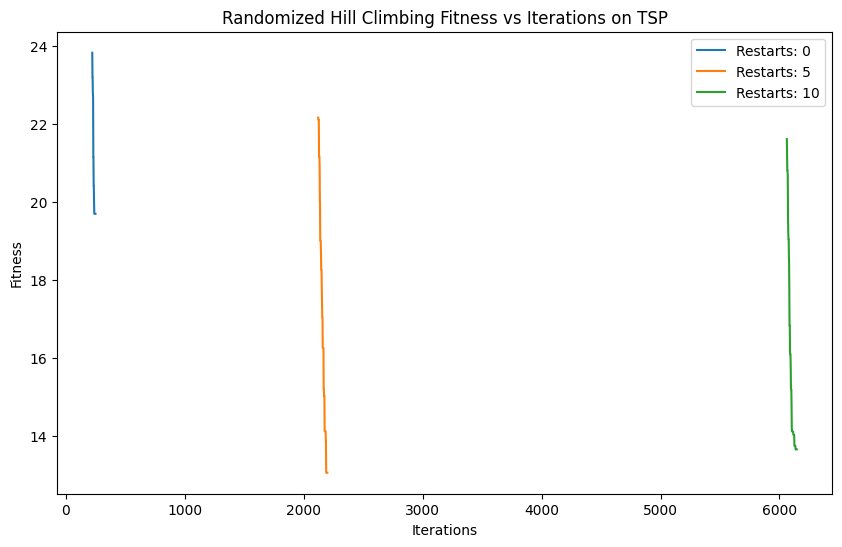
\includegraphics[width=\textwidth]{image/part-2/rhc.png}
        \caption{}
        \label{fig:2rhc}
    \end{subfigure}
    \vskip\baselineskip
    \begin{subfigure}[b]{0.49\textwidth}
        \centering
        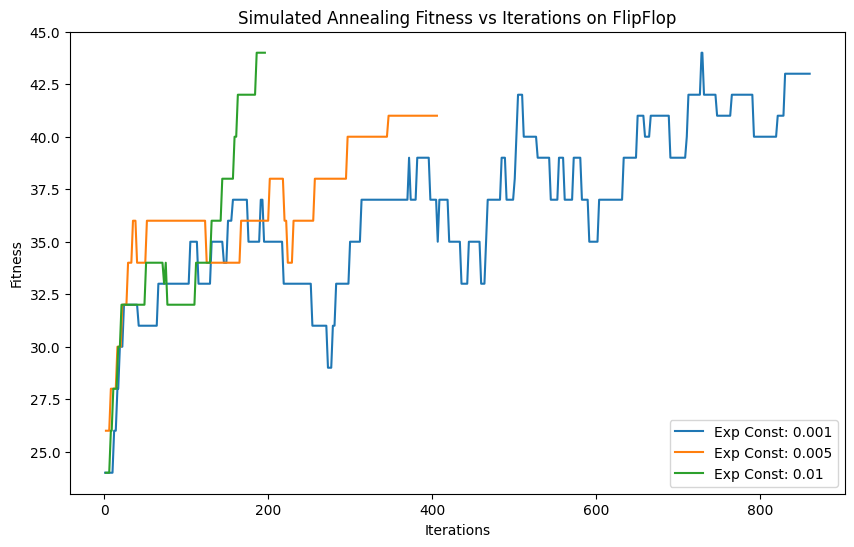
\includegraphics[width=\textwidth]{image/part-2/sa.png}
        \caption{}
        \label{fig:2sa}
    \end{subfigure}
    \hfill
    \begin{subfigure}[b]{0.49\textwidth}
        \centering
        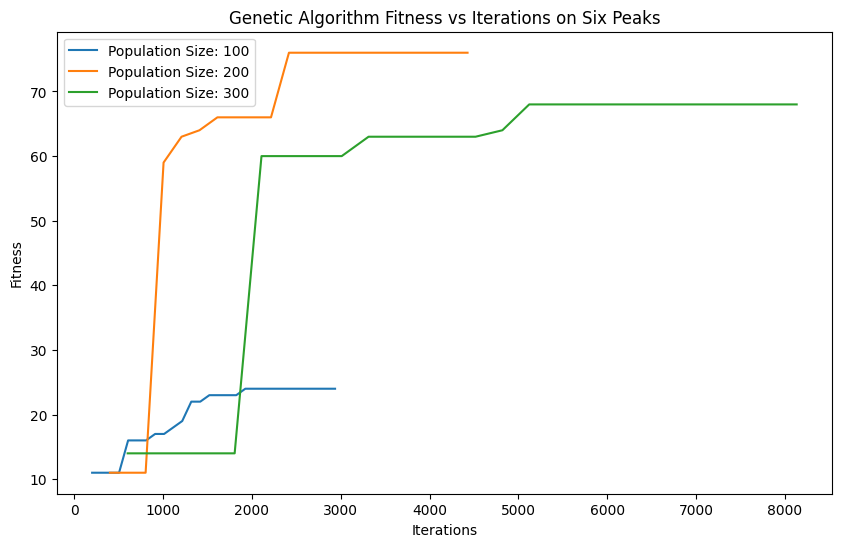
\includegraphics[width=\textwidth]{image/part-2/ga.png}
        \caption{}
        \label{fig:2ga}
    \end{subfigure}
    \caption{Comparison of learning curves for training a Neural Network using different optimization algorithms: (a) Backpropagation, (b) Randomized Hill Climbing, (c) Simulated Annealing, and (d) Genetic Algorithm. Backpropagation demonstrates smooth convergence with minimal fluctuations, while the randomized optimization algorithms (RHC, SA, GA) show varying degrees of instability, especially in early iterations.}
    \label{fig:2grid}
\end{figure*}

\begin{figure}[htbp]
\centerline{\includegraphics[width=1\linewidth]{image/part-2/best.png}}
\caption{Comparison of best learning curves for Neural Network training using backpropagation, Randomized Hill Climbing (RHC), Simulated Annealing (SA), and Genetic Algorithm (GA).}
\label{fig:2best}
\end{figure}

\begin{figure}[htbp]
    \centering
    \begin{subfigure}[b]{0.48\textwidth}
        \centering
        \includegraphics[width=\textwidth]{image/part-2/best accuracy.png}
        \caption{}
        \label{fig:2accuracy}
    \end{subfigure}
    \vskip\baselineskip
    \begin{subfigure}[b]{0.48\textwidth}
        \centering
        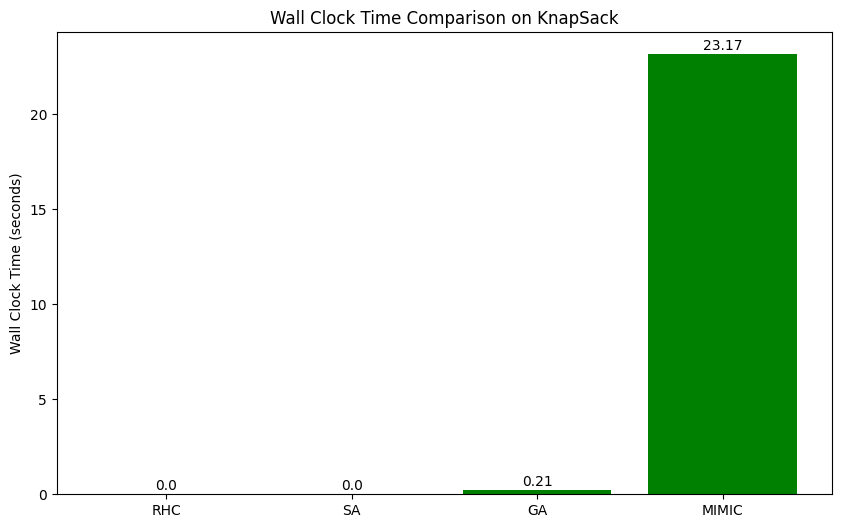
\includegraphics[width=\textwidth]{image/part-2/time.png}
        \caption{}
        \label{fig:2time}
    \end{subfigure}
    \caption{Comparison of the best accuracy and wall clock time for Neural Network training across different optimization algorithms. While Backpropagation is the fastest, SA achieves the best accuracy, though it is the slowest in terms of time. RHC and GA show moderate accuracy but take significantly longer compared to Backpropagation.}
    \label{fig:2accuracytime}
\end{figure}